\section{Ejercicio 1}

En este ejercicio tenemos alumnos que desean ir a cualquier escuela en su barrio y nosotros como departamento de computación queremos interceptarlos para contarles sobre la carrera. Para eso queremos poner a estudiantes de la carrera de manera tal que no haya manera que ningún alumno nos pueda esquivar.

Tenemos entonces tres tipos de esquinas en la ciudad. Las que tienen la casa de algún alumno, las que tienen una escuela y aquellas que están desocupadas.

\begin{figure}[h]
  \centering
    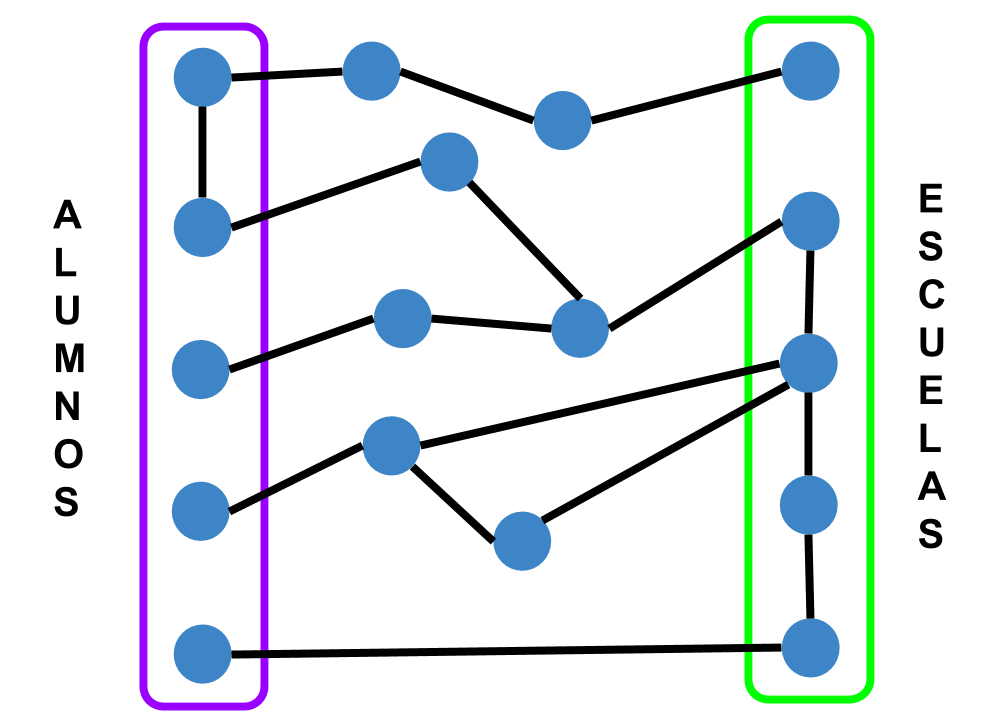
\includegraphics[scale = 0.225]{img/esquema.png}
    \caption{Grafo G}
\end{figure}

Como se aprecia en la figura anterior tenemos dos conjuntos importantes, las casas de los alumnos y las escuelas. Vale destacar que estos son disjuntos puesto que por enunciado una esquina puede ser de un solo tipo.

\subsection{Modelando el problema}

La entrada del problema, es decir las calles y las esquinas con sus tipos nos definen un grafo G = (V,E). Este grafo es conexo ya que desde cualquier esquina se puede llegar a cualquier otra. Definamos A como el subconjunto de vértices donde se encuentran los alumnos y C como el subconjunto de vértices donde se encuentran las escuelas(C por colegios).

Lo que buscamos es tomar un subconjunto de V de manera tal que para cualquier camino de un nodo que pertenece a A hacia un nodo que pertenece a C pase por algún nodo de ese subconjunto buscado. En particular buscamos que ese subconjunto sea mínimo.

Para lograrlo definamos G', el grafo que se define como G'= (V',E') con V' = V $\cup$ $\{s,t\}$ y E' = E $\cup$ $\{(x,y)| x = s, x \in V , x \in Alumnos \}$ $\cup$ $\{(x,y)| y = t, x \in V , x \in Escuelas \}$.

\begin{figure}[h!]
  \centering
    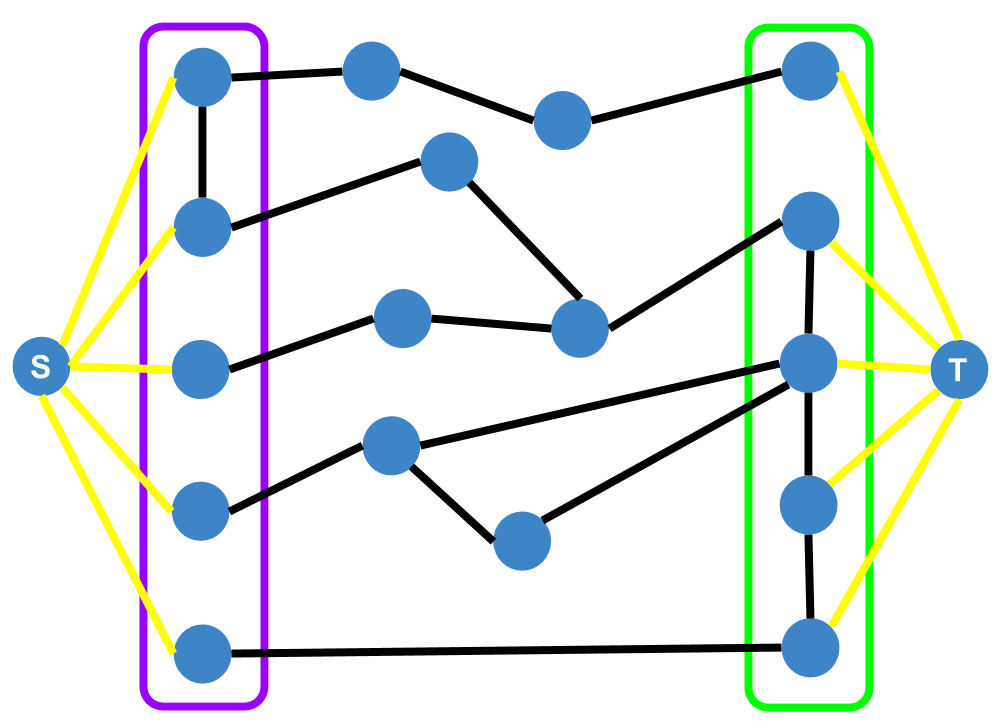
\includegraphics[scale = 0.225]{img/gprima.png}
    \caption{Grafo G'}
\end{figure}

En palabras sería tomar el grafo anterior y agregarle dos nodos más, uno de ellos conectado a todas las escuelas y el otro conectado a todos los alumnos.


\par{Afirmamos que buscamos la minima cantidad de vertices tal que al removerlos, no haya camino de una un estudiante a una escuela. 
Esto es asi ya que, si al removerlos nodos, deja de haber camino, quiere decir que cualquier camino de una estudiante a una escuela usaba por lo menos uno de estos vertices. 
Entonces podemos usar a estos mismos como lugares para posicionarnos, y cubrimos todos los caminos, que es lo que queríamos. Ademas si sacamos menos que estos vertices, sigue habiendo por lo menos un camino de un un Estudiante  a una Escuela que no utiliza ninguno de estos vértices, por definicion. Entonces posicionarnos en menos lugares no nos sirve. }
\par{
Asi demostramos que nuestro problema es equivalente a la minima cantidad de vertices que desconecta las escuelas de los estudiantes. 
Como todo camino de s a t (source y sink de G’) tiene como subcamino un camino de escuela a un estudiante, y todo camino de escuela a estudiante es subcamino de s a t, entonces es equivalente a buscar la mínima cantidad de vertices de G’ tal que al removerlos deja a s y t en dos componentes conexas distintas.}
\par{
Esto es exactamente igual a lo que se como “mínimo corte sobre los vertices que desconecta a s y t”. Llamado en inglés, minimum vertex cut.
Ahora, una vez más, volvemos a reducir el problema. El “minimun vertex cut”  sobre s y t, es equivalente a la máxima cantidad de caminos disjuntos en vértices desde s a t, gracias al Teorema de Menger.}

\subsection{Algoritmo para encontrar máxima cantidad de caminos disjuntos en un grafo}

Por lo dicho anteriormente, queremos encontrar la máxima cantidad de caminos disjuntos. De nuevo, vamos a seguir extendiendo el grafo para que tenga las 
propiedades buscadas. Sea G'' un digrafo.
Como por un nodo `x' de G puede pasar tantas unidades de flujo como sucesores directos tenga (como cota superior) en el grafo, la idea será duplicar al nodo en dos partes. Por un lado tenemos el nodo `x$_{in}$' al cual se le conectarán todas las aristas de los predecesores directos
 y por el otro tenemos a `x$_{out}$' del cual saldrán las aristas correspondientes a los sucesores directos. 
Si la única arista que sale de `x$_{in}$' va a `x$_{out}$' 
entonces, aunque `x' tenga muchos sucesores directos a los cuales está conectado en G o G', en el nuevo grafo G'' solo podrá dejar pasar flujo a uno de ellos puesto que la arista entre sus dos nuevas partes lo limita a tan solo uno.
Es decir, G'' es un digrafo que tiene, para cada vértice x de G, dos vértices x$_{in}$' y `x$_{out}$, anteriormenete descriptos. Además, tiene los mismos vértices s y t de G', 
donde s se conecta a todos los x$_{in}$' correspondientes a los alumnos. Por otro lado t tiene una arista entrante desde todos los `x$_{out}$ correspondientes a las escuelas. 
Estos vértices son todos los vértices que contiene G''. 
Las aristas de G'' son aquellas aristas que teníamos en G', de x a y, pero de x$_{out}$' a `y$_{in}$, más las aristas del source y sink (s y t), más las aristas de x$_{in}$' a `x$_{out}$. Estas son todas las aristas.
Todas las aristas tendran capacidad 1.

\par{Vamos a ver que un flujo máximo sobre G'' es igual a la máxima cantidad de caminos de s a t, disjuntos en vértices.
Sea f un flujo en G''. El flujo |f| es igual a la cantidad de aristas que llegan a t, tal que f(e) = 1. Si tomamos una arista e, desde x$_{out}$ a t, podemos ver que, el flujo
hasta x$_{out}$ es igual a 1, pues sale flujo de ella, y no llega mas de una arista. Entonces vamos a x$_{in}$, cuyo flujo es 1, ya que no sale mas de una arista de x$_{in}$.
Asi podemos iterar hasta llegar a s, con lo cual tenemos un camino en G''. Como ninguna de estas aristas puede usarse en dos caminos, porque sus capacidades son 1,
entonces tenemos caminos disjuntos en G''. Ademas, para cada camino en G'' podemos construir un camino distinto en G', porque si no, tendriamos aristas de G'' que van a parar a las mismas aristas o vértices de G', lo cual es falso. 
Entones el valor del flujo |f| nos da una cantidad de caminos disjuntos en G'' y en G'. 
Además, análogamente, si tenemos caminos disjuntos en G'', podemos definir un flujo, cuyo valor |f| es igual al cardinal del conjunto de caminos. Es decir, hay una biyección entre
los flujos distintos y los caminos disjuntos en vértices.
Entonces si f es flujo máximo, |f| nos da la máxima cantidad de caminos disjuntos en G' o en G'', que es lo que queríamos. }

\subsection{Resolución al problema}

Como primer paso entonces debemos construir el grafo (digrafo) de manera tal que para cada arista e = (a,b), e $\in$ E, conectamos `a$_{out}$' con `b$_{in}$' y `b$_{out}$' con `a$_{in}$'.

Luego, hay que agregar los nodos s y t que usábamos para el grafo G'. Entonces conectamos s con todo vértice `v$_{in}$' si v $\in$ A y a todo vértice `w$_{out}$' con t si w $\in$ C.

Ahora sí, ya tenemos nuestro digrafo construido al que tenemos que aplicarle un algoritmo de flujo máximo que nos dará la respuesta que buscamos.

\subsection{Respetando las complejidades}

Para construir el grafo utilizamos una lista de adyacencia la cual usaremos luego también como red residual. Es por eso que al conectar un nodo con otro en la lista de adyacencia, no solo agregamos cual es dicho vecino sino también la capacidad que tiene dicha arista (en nuestro caso todas las aristas comienzan con capacidad 1). Esto tiene complejidad \bigo(M+N) puesto que todas las aristas del grafo las agregamos dos veces en nuestro digrafo y las aristas a los dos supernodos (s y t) son a lo mucho N (en el caso donde todos los nodos son escuelas o alumnos). 

El algoritmo de flujo máximo elegido es Edmons Karp que como bien vimos en clase tiene complejidad \bigo$(M^2 \times N)$.

Por lo tanto la complejidad total está dominada por el algoritmo de flujo y nuestro problema tiene complejidad temporal total de \bigo$(M^2 \times N)$

\subsection{Pseudocódigo}
	
\begin{algorithmic}
\Function{calcular$\_$camino$\_$aumento}{capacidad_red_residual, G, source, sink}
	\State cola c, visited[tamaño(G)] = [false .. false], padre[tamaño(G)] = [-1 .. -1]
	\State c.encolar(source)
	
	\Comment{BFS}

	\While{not cola.vacía}
		\State actual $\leftarrow$ cola.tope()
		\State cola.desencolar
		
		\State visited[actual] $\leftarrow$ true
	
		\For{v : adj[actual]} \Comment{Para cada vecino del nodo actual en G}
				\If {not visited[v] and capacidad_red_residual[actual][v] == 1}
					\State p[v] $\leftarrow$ actual
					\State cola.encolar(v)
				\EndIf
		\EndFor 
	\EndWhile

	\If{not visited[sink]} 
		\State \Return 0 \Comment{Si no hubo camino de aumento (no llegué al nodo final)}
	\EndIf

	\Comment{Caso contrario reconstruyo el camino y reconstruyo la capacidad de la red residual.}
	\State actual $\leftarrow$ sink
	\State padre $\leftarrow$ p[actual]
	
	\While{padre!=-1}
		\State capacidad_red_residual[padre][actual] $\leftarrow$ 0
		\State capacidad_red_residual[actual][padre] $\leftarrow$ 1
		
		\State actual $\leftarrow$ padre
		\State padre $\leftarrow$ p[actual]
	\EndWhile

	\State \Return 1 \Comment{Toda arista tiene capacidad 1.}
\EndFunction
\end{algorithmic}
\hspace{1cm}

\begin{algorithmic}
\Function{flujo$\_$máximo}{capacidad_red_residual, G,source, sink}
	\State flujo$\_$total $\leftarrow$ 0
	\Repeat 
			\State aumentar $\leftarrow$ calcular$\_$camino$\_$aumento(capacidad_red_residual, G, source,sink)
			\State flujo$\_$total = flujo$\_$total + aumentar
	\Until{aumentar $\neq$ 0}
	
\EndFunction
\end{algorithmic}
\hspace{1cm}

\begin{algorithmic}
\Function{conectar}{capacidad_red_residual, G, A, B}
	\State capacidad_red_residual [a][b] $\leftarrow$ 1
	\State conectar A con B en G
	\State conectar B con A en G
\EndFunction
\end{algorithmic}
\hspace{1cm}

\begin{algorithmic}
\Function{main}{N, M, tipo$\_$esquina T[], lista$\_$incidencia L[]}
	\State \textit{\textbf{Vamos a tener a todo nodo del grafo original duplicado como V$_{entrante}$ y V$_{saliente}$}}
	\State \textit{\textbf{Y el digrafo representado como una lista de adyacencia.}}
	\State \textit{\textbf{Por otro lado la red residual como una matriz de Tamaño(G) * Tamaño(G)}}
	\State \textit{\textbf{Y como las capacidades en la red residual 0 o 1, entonces al generar caminos de aumento se simplificará para que devuelva 1 de aumento en el flujo si hay camino y 0 caso de que no.}}
	\State Tamaño(G) = 2 * N + 2
	\State capacidad_red_residual [Tamaño(G)][Tamaño(G)] $\leftarrow$ [0 .. 0] 
	\State source $\leftarrow$ 0, sink $\leftarrow$ 2*N+1
	\For{tipo$\_$esquina t : T}
		\If{t = Escuela}
			\State conectar(capacidad_red_residual, G, t$_{saliente}$, sink) 
		\Else{
			\If{t = Alumno}
				\State conectar(capacidad_red_residual, G, source, t$_{entrante}$)
			\EndIf
		}
		\EndIf
	\EndFor
	\For{v $\leftarrow$ [1..N]}
		\State conectar(capacidad_red_residual, G, v$_{entrante}$, v$_{saliente}$)
	\EndFor

	\For{arista a : L}
		\State v = extremo_izquierdo, w = extremo_derecho
		\State conectar(capacidad_red_residual, G, v$_{saliente}$, w$_{entrante}$)
		\State conectar(capacidad_red_residual, G, w$_{saliente}$, v$_{entrante}$)
	\EndFor
	
	\Return flujo$\_$máximo(capacidad_red_residual, G, source, sink)

\EndFunction

\end{algorithmic}


